% !TeX program = xelatex
\documentclass[12pt,a4paper]{article}

% =========================================================
% 0) XeLaTeX + 中英文兼容（英文默认 Times New Roman）
% =========================================================
\usepackage{iftex}
\ifXeTeX\else
\errmessage{This template requires XeLaTeX. Please compile with XeLaTeX.}
\fi

\usepackage{fontspec}
\usepackage{xeCJK}

% ---- 英文字体：Times New Roman（无则回退）----
\IfFontExistsTF{Times New Roman}{%
	\setmainfont{Times New Roman}%
}{%
	\setmainfont{TeX Gyre Termes}%
}
\IfFontExistsTF{Arial}{\setsansfont{Arial}}{\setsansfont{TeX Gyre Heros}}
\IfFontExistsTF{Menlo}{\setmonofont{Menlo}}{\setmonofont{Latin Modern Mono}}

% ---- 中文字体：mac 常见字体自动回退（无则兜底 Fandol）----
\IfFontExistsTF{Songti SC}{\setCJKmainfont{Songti SC}}{
	\IfFontExistsTF{STSong}{\setCJKmainfont{STSong}}{
		\IfFontExistsTF{PingFang SC}{\setCJKmainfont{PingFang SC}}{
			\IfFontExistsTF{Hiragino Sans GB}{\setCJKmainfont{Hiragino Sans GB}}{
				\IfFontExistsTF{Noto Serif CJK SC}{\setCJKmainfont{Noto Serif CJK SC}}{
					\IfFontExistsTF{Source Han Serif SC}{\setCJKmainfont{Source Han Serif SC}}{
						\setCJKmainfont{FandolSong-Regular}
					}
				}
			}
		}
	}
}
\IfFontExistsTF{PingFang SC}{\setCJKsansfont{PingFang SC}}{}
\IfFontExistsTF{STHeiti}{\setCJKsansfont{STHeiti}}{}
\IfFontExistsTF{Songti SC}{\setCJKmonofont{Songti SC}}{}

% =========================================================
% 1) 页面布局 & 排版
% =========================================================
\usepackage[a4paper,margin=2.5cm]{geometry}
\usepackage{microtype}
\usepackage{setspace}
\setstretch{1.25}
\usepackage{indentfirst}
\setlength{\parindent}{2em}
\setlength{\parskip}{0.3em}

% =========================================================
% 2) 数学 & 符号
% =========================================================
\usepackage{amsmath,amssymb,amsthm,mathtools}
\usepackage{bm}
\usepackage{siunitx}
\sisetup{per-mode=symbol,detect-all}

% ---- 定理环境 ----
\theoremstyle{plain}
\newtheorem{theorem}{Theorem}[section]
\newtheorem{lemma}[theorem]{Lemma}
\newtheorem{proposition}[theorem]{Proposition}
\newtheorem{corollary}[theorem]{Corollary}

\theoremstyle{definition}
\newtheorem{definition}[theorem]{Definition}
\newtheorem{example}[theorem]{Example}
\newtheorem{problem}[theorem]{Problem}

\theoremstyle{remark}
\newtheorem{remark}[theorem]{Remark}
\newtheorem*{note}{Note}

% ---- 常用算子（ML/NLP 友好）----
\DeclareMathOperator*{\argmax}{arg\,max}
\DeclareMathOperator*{\argmin}{arg\,min}
\DeclareMathOperator{\softmax}{softmax}
\DeclareMathOperator{\tr}{tr}
\DeclareMathOperator{\rank}{rank}
\DeclareMathOperator{\diag}{diag}
\DeclareMathOperator{\sgn}{sgn}
\DeclareMathOperator*{\E}{\mathbb{E}}
\DeclareMathOperator*{\Var}{Var}
\DeclareMathOperator*{\Cov}{Cov}

% ---- 常用集合简写 ----
\newcommand{\R}{\mathbb{R}}
\newcommand{\N}{\mathbb{N}}
\newcommand{\Z}{\mathbb{Z}}
\newcommand{\Q}{\mathbb{Q}}
\newcommand{\C}{\mathbb{C}}

% ---- 配对定界符（自动缩放）----
\DeclarePairedDelimiter{\abs}{\lvert}{\rvert}
\DeclarePairedDelimiter{\norm}{\lVert}{\rVert}
\DeclarePairedDelimiter{\ceil}{\lceil}{\rceil}
\DeclarePairedDelimiter{\floor}{\lfloor}{\rfloor}
\DeclarePairedDelimiter{\inner}{\langle}{\rangle}
% 用法：\abs{x}、\norm*{Ax} （带 * 会自动匹配大小）

% =========================================================
% 3) 颜色 & 图形
% =========================================================
\usepackage[dvipsnames,table]{xcolor}

\usepackage{graphicx}
\usepackage{float}
\usepackage{subcaption}

% ---- TikZ + 常用库 ----
\usepackage{tikz}
\usetikzlibrary{
	arrows.meta,
	positioning,
	calc,
	shapes.geometric,
	shapes.misc,
	fit,
	matrix,
	trees,
	decorations.pathreplacing,
	decorations.markings,
	patterns,
	backgrounds,
	3d
}

% ---- pgfplots（画函数/数据图）----
\usepackage{pgfplots}
\pgfplotsset{compat=1.18}
\usepgfplotslibrary{fillbetween}

% =========================================================
% 4) 算法伪代码
% =========================================================
\usepackage{algorithm}
\usepackage{algpseudocode}
% 常用命令：\begin{algorithm} / \begin{algorithmic}[1]
		% \State \If \ElsIf \Else \EndIf \For \While \Function \Return

		% =========================================================
		% 5) 代码高亮（listings，XeLaTeX 友好）
		% =========================================================
		\usepackage{listings}
		\definecolor{codebg}{RGB}{248,248,248}
		\definecolor{codekw}{RGB}{0,0,180}
		\definecolor{codestr}{RGB}{163,21,21}
		\definecolor{codecom}{RGB}{0,128,0}
		\definecolor{codenum}{RGB}{128,128,128}
		\lstset{
			basicstyle=\ttfamily\small,
			backgroundcolor=\color{codebg},
			keywordstyle=\color{codekw}\bfseries,
			stringstyle=\color{codestr},
			commentstyle=\color{codecom}\itshape,
			numberstyle=\tiny\color{codenum},
			numbers=left,
			numbersep=6pt,
			frame=single,
			framerule=0pt,
			breaklines=true,
			breakatwhitespace=true,
			showstringspaces=false,
			tabsize=2,
			captionpos=b,
			columns=fullflexible,
			keepspaces=true,
			extendedchars=true,
			xleftmargin=1em,
			xrightmargin=0.5em,
			aboveskip=0.8em,
			belowskip=0.8em,
		}
		% 预置几个常用语言别名
		\lstdefinestyle{py}{language=Python}
		\lstdefinestyle{cpp}{language=C++}
		\lstdefinestyle{bash}{language=bash}

		% =========================================================
		% 6) 表格
		% =========================================================
		\usepackage{booktabs}
		\usepackage{tabularx}
		\usepackage{multirow}
		\usepackage{makecell}
		\usepackage{array}
		\usepackage{longtable}

		% =========================================================
		% 7) 列表 & 引用 & 杂项
		% =========================================================
		\usepackage{enumitem}
		\setlist{noitemsep,topsep=0.3em}

		\usepackage{csquotes}   % 智能引号 \enquote{...}
		\usepackage{url}
		\usepackage{appendix}

		\usepackage{caption}
		\captionsetup{font=small,labelfont=bf}

		% =========================================================
		% 8) 超链接 & 交叉引用（hyperref 几乎放最后，cleveref 放 hyperref 之后）
		% =========================================================
		\usepackage{hyperref}
		\hypersetup{
			colorlinks=true,
			linkcolor=blue,
			urlcolor=blue,
			citecolor=blue,
			bookmarksnumbered=true,
			bookmarksopen=true,
			pdfencoding=auto
		}

		\usepackage[capitalize,noabbrev]{cleveref}
		% 用法：\cref{eq:loss} 自动输出 "Eq. (1)"；\Cref 句首大写

		% =========================================================
		% 9) 文档信息
		% =========================================================
		\title{Echo: Midterm Progress Report}
		\author{Lingchao Nie, Fanghui Xu, Yuqing Zhou \\ \small Westlake University}
		\date{\today}

		\begin{document}
			\maketitle

			\textbf{Team members:} Lingchao Nie, Fanghui Xu, Yuqing Zhou (Westlake University).

			\section{Project introduction}

			Hermes Agent is an open-source AI assistant that uses tools and learns reusable ``skills'' from past sessions. Our proposal pointed out three problems in how Hermes manages those skills: (1) the agent grades its own work, so feedback is biased; (2) a new skill is created only when the agent has called many tools, which misses many useful cases; (3) once saved, there is no record of when a skill should \emph{not} apply. Echo is a Hermes plugin that addresses all three. It collects user-behaviour signals during a session, runs them through a confidence engine and a drift detector, and feeds the result back into how Hermes picks and reuses skills. Five modules cover this end to end (M1--M5, see Figure~\ref{fig:arch}).

			\begin{figure}[H]
				\centering
				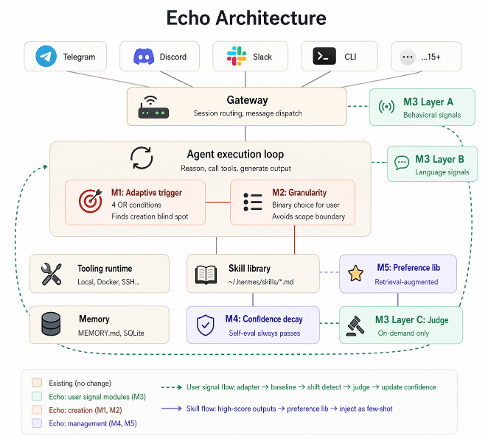
\includegraphics[width=0.78\linewidth]{Echo.png}
				\caption{Echo's architecture. The beige blocks --- M1, M2, M4, M5, and the three Layer~A/B/C signal channels --- are the parts Echo adds on top of Hermes.}
				\label{fig:arch}
			\end{figure}

			\section{Current status}

			All five modules M1--M5, the web dashboard, and a Tauri-based desktop shell are implemented as a Hermes plugin, without modifying any core file. M1 nominates an invocation as ``worth saving as a skill'' when any of four conditions fire (save-intent regex, $\geq 5$ tool calls, $\geq 3$ modification rounds, or repeated similar requests). M2 asks the user a binary scope question at the bottom of the chat tab whenever a new skill is created. M3 keeps a Welford running mean and variance per (skill, metric) and flags $|z|\geq 2$ as drift. M4 turns every incoming signal into a single $[0,1]$ confidence score (Section~\ref{sec:fb}). M5 stores good past examples as embeddings and injects retrieved few-shots into the user message --- not the system prompt --- so Hermes' prompt cache stays valid. Tests: 365 Echo unit tests plus a 34-step end-to-end smoke test pass on every commit, alongside 69 existing Hermes plugin-discovery tests --- no upstream regression.

			\section{Feedback mechanism and signal fusion}\label{sec:fb}

			The proposal review asked us to make the feedback mechanism concrete. It is now \emph{eight} channels in three families.

			\textbf{Explicit (user clicks).} (i) \emph{Thumbs $\pm 1$} at the chat bottom: short tap submits ${\pm}1$, long press ($\geq 500$\,ms) opens a textarea for an optional reason; a $+1$ also seeds the M5 preference library so the same turn can be retrieved as a few-shot example next time. (ii) \emph{A/B scope question} for each new skill: a binary choice between ``reuse broadly'' and ``only the general idea'', recorded for the M5 retriever.

			\textbf{Implicit (no clicks).} (iii) \emph{Tool-call count} and (iv) \emph{modification-round count} per invocation, both collected from plugin hooks. (v) \emph{Drift detection} turns those counters into a signed signal via the Welford statistics above. (vi) \emph{Layer~B sentiment}: every user turn is classified by an auxiliary LLM as positive / negative / neutral, with a prompt deliberately biased toward neutral so ambiguous wording does not move $c$. (vii) \emph{Desktop signals} from the Tauri shell: OS clipboard changes and window focus/blur events --- two sources a normal browser tab cannot see.

			\textbf{LLM audit.} (viii) \emph{Layer~C judge.} At every \emph{active $\rightarrow$ pending\_review} transition --- and only then, so cost stays bounded --- a separate LLM reads the recent transcript and returns one of \texttt{ok}, \texttt{degraded} (extra penalty), or \texttt{exclusion} (a machine-readable rule appended to the skill's scope). Because the judge is a separate instance with no shared state, this directly addresses the same-source self-evaluation bias.

			\paragraph{Fusion into one number.} Each channel emits one event $e = (\text{skill}, T, s)$, where $T$ is the rule type and $s \geq 1$ is severity. Per-skill confidence $c \in [0,1]$ updates event-by-event:
			\[
				c \;\leftarrow\; \mathrm{clip}_{[0,1]}\bigl(g_T(c,s)\bigr),\qquad
				g_T(c,s) =
				\begin{cases}
					c + \alpha_T, & T \in \{\text{explicit+},\ \text{NL+}\} \quad \text{(additive boost)} \\
					c\,(1 - \beta_T\, s), & T \in \{\text{explicit-},\ \text{NL-},\ \text{drift}\} \quad \text{(multiplicative penalty)} \\
					c, & T = \text{silence (sacred invariant)}
				\end{cases}
			\]
			The lifecycle state is read off $c$ alone: \emph{active} for $c \geq 0.30$, \emph{pending\_review} for $0.10 \leq c < 0.30$ (this triggers the Layer~C judge), \emph{retired} (sticky) for $c < 0.10$. Current values: $\alpha_{\text{exp+}}{=}0.10$, $\alpha_{\text{NL+}}{=}0.05$, $\beta_{\text{exp-}}{=}0.30$, $\beta_{\text{NL-}}{=}0.15$, $\beta_{\text{drift}}{=}0.15$; $s{=}1$ for explicit/NL rules and $s{=}\min(|z|, 3)$ for drift. The two-family form is on purpose: additive boosts let several positive signals accumulate without saturating, while multiplicative penalties make a single strong negative bite hard and small repeated negatives compound geometrically. The implicit and desktop channels feed this same update through drift, so all eight channels move the same scalar $c$ on the same $[0,1]$ scale. The hyperparameters above, the warm-up window, the state thresholds, and the long-press / polling intervals are all still being tuned --- the current set is a working hypothesis, not the final answer.

			\section{Plan and challenges}

			The remaining work is empirical, over roughly four weeks: (1) build a deterministic simulated user that drives Hermes through scripted sessions with planted ground truth about which skills should fire, drift, or retire; (2) run plain Hermes and Hermes+Echo (plus an ablation with the confidence engine disabled) as baselines; (3) measure four numbers --- M1 nomination precision against Hermes' ``$\geq 5$ tool calls'' rule, M3 drift precision/recall on planted distribution shifts, M4 Spearman $\rho$ between $c$ and a held-out ``true usefulness'' signal, M5 task-success uplift from few-shot injection (on vs. off); (4) write up and record a short walkthrough. Three challenges we expect: making the simulated user realistic enough to exercise Layer~B sentiment (we plan paraphrased templates and a small noise model), keeping Layer~B/C LLM costs reproducible (record-and-replay), and defining ``true usefulness'' cleanly enough that M4 calibration is meaningful.

		\end{document}
